\documentclass[a4paper,11pt]{article}
\usepackage{ls}
\usepgfplotslibrary{patchplots}

\pagestyle{empty}
\begin{document}

\begin{center}
  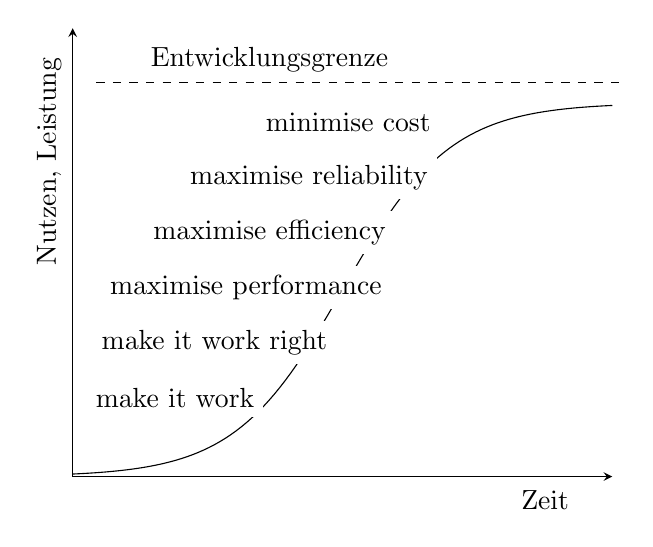
\begin{tikzpicture}
    \begin{axis}[
        xmin=0, xmax=10, ymin=0,ymax=12,
        axis lines=middle,
        xtick={\empty},ytick={\empty},
      ]
      \addplot[samples=100,domain=0:10] expression {10/(1+exp(-(x-5))) } ;
    \end{axis}
    \node[rotate=90] at (-.3,4) {Nutzen, Leistung} ;
    \node[] at (6,-.3) {Zeit} ;
    \node[] at (2.5,5.3) {Entwicklungsgrenze}; 
    \draw[-,dashed] (0.3,5) -- (7,5) ;
    \node[fill=white] at (1.3,1) {make it work} ;
    \node[fill=white] at (1.8,1.7) {make it work right} ;
    \node[fill=white] at (2.2,2.4) {maximise performance} ;
    \node[fill=white] at (2.5,3.1) {maximise efficiency} ;
    \node[fill=white] at (3,3.8) {maximise reliability} ;
    \node[fill=white] at (3.5,4.5) {minimise cost} ;
  \end{tikzpicture}\\[1em]
  Entwicklungsschritte entlang der S-Kurve am Beispiel Verbrennungsmotor
\end{center}
\end{document}
